\documentclass{article}
\usepackage[utf8]{inputenc}
\usepackage[T1]{fontenc}
\usepackage{array}
\usepackage{longtable}
\usepackage[spanish]{babel}
\usepackage{geometry}
\usepackage{booktabs} 
\usepackage{amsmath}
\usepackage{graphicx}
\usepackage{subfigure}
\usepackage{float}
\usepackage{caption}
\usepackage[section]{placeins}
\usepackage{multicol}

\geometry{
 a4paper,
 margin=2.5cm,
}

\title{Revisión de Estrategias de Almacenamiento de Hidrógeno en Hidruros Metálicos: Gestión Térmica y Diseño de Tanques}
\author{pre- informe  Matriz de Información}
\date{\today}

\begin{document}

\maketitle

\begin{abstract}
Este documento presenta una introducción al almacenamiento de hidrógeno ($\text{H}_2$) en estado sólido, centrándose en la **gestión de la transferencia de calor** como el desafío central en los reactores de hidruros metálicos (MH). Se destaca el proceso de absorción exotérmica y desorción endotérmica, cuyo rendimiento dinámico está intrínsecamente ligado al diseño del intercambiador de calor. Posteriormente, se compila la información de estudios clave sobre el diseño de tanques, los materiales de hidruro y las estrategias de modelado, prestando especial atención a la comparación de diferentes configuraciones de enfriamiento.
\end{abstract}

\section{Introducción: El Desafío de la Transferencia de Calor en Hidruros Metálicos}

El **hidrógeno ($\text{H}_2$)** es un vector energético crucial para la descarbonización global. Entre las diversas tecnologías para su almacenamiento, los **hidruros metálicos (MH)** ofrecen una de las soluciones más seguras y compactas, ya que almacenan $\text{H}_2$ en estado sólido a presiones y temperaturas moderadas.

Sin embargo, el uso de MH presenta una limitación significativa: la **gestión térmica**. La reacción de **absorción de hidrógeno** es fuertemente **exotérmica** (libera calor), mientras que la **desorción** es **endotérmica** (requiere calor). Para lograr tasas rápidas de carga (absorción) y descarga (desorción) de $\text{H}_2$, es imprescindible diseñar un sistema de intercambio de calor eficiente que pueda disipar rápidamente el calor generado o suministrar el calor requerido.

En este contexto, la **optimización del diseño del reactor (tanque)** y la incorporación de **intercambiadores de calor (HE)** se convierten en el foco principal de la investigación. Estudios como el de **Satya Sekhar et al. (2015)** demuestran que el rendimiento dinámico del almacenamiento está determinado esencialmente por la intensidad del intercambio de calor entre el fluido de transferencia de calor (HTF) y el lecho de hidruro, haciendo que la selección del \textbf{layout} óptimo del tanque sea un factor determinante.

\section{Estudios Clave sobre Diseño de Reactores y Gestión Térmica}

La siguiente tabla resume varios estudios que exploran diferentes estrategias de diseño de reactores, materiales y modelado enfocadas en mejorar la transferencia de calor en sistemas de almacenamiento de hidruros metálicos.

\begin{table}[!ht]
\centering
\caption{Resumen de Artículos Clave sobre Diseño de Reactores de Hidruros Metálicos}
\label{tab:resumen_hidruros}

\begin{tabular}{>{\raggedright}m{2.5cm}|>{\raggedright}m{2.5cm}|>{\raggedright}m{3.5cm}|>{\raggedright}m{2.5cm}|>{\raggedright\arraybackslash}m{4cm}}
\toprule
\textbf{Referencia (Año)} & \textbf{Material de Hidruro} & \textbf{Diseño de Tanque/Estrategia} & \textbf{Modelo/Simulación} & \textbf{Hallazgos Principales} \\
\midrule

2007: High Density Hydrogen Storage System Demonstration & $\text{NaAlH}_4$ (Hidruro complejo) & Recipientes de \textbf{fibra de carbono} para alta presión y gestión del calor con **aceite inerte**. & Ecuaciones de transferencia de calor y FEA (Análisis de Elementos Finitos). & El diseño con un \textbf{intercambiador de calor} y un recipiente compuesto es viable para el \textbf{almacenamiento de alta densidad}. \\
\midrule
2008: Optimization of hydrogen storage in metal-hydride tanks & No especificado (estudio general) & Tanque cilíndrico comparado con diseños con \textbf{aletas externas} y \textbf{tubos internos} (concéntricos o en U). & Modelo matemático 2D validado experimentalmente. & El uso de \textbf{aletas} y \textbf{tubos internos} (como en los diseños con tubos en U) \textbf{mejora significativamente la transferencia de calor} y reduce el tiempo de almacenamiento. \\
\midrule
\textbf{2015: Performance Analysis of Cylindrical Metal Hydride Beds} & $\text{MmNi}_{4.6}\text{Al}_{0.4}$ (Aleación $\text{AB}_5$) & Comparación de 4 \textbf{layouts} de enfriamiento: \textbf{(I)} Tubo recto interno, \textbf{(II)} Tubo helicoidal, \textbf{(III)} Enfriamiento externo, \textbf{(IV)} Enfriamiento externo con aletas transversales. & Modelo numérico \textbf{3D de transferencia de calor y masa} con \textbf{COMSOL Multiphysics}. & La comparación dinámica de las 4 configuraciones es crucial. La \textbf{intensidad del intercambio de calor} entre el $\text{HTF}$ y el $\text{MH}$ es el principal factor que determina la velocidad de carga/descarga de $\text{H}_2$. \\
\midrule
2017: Impact of using a heat transfer fluid pipe in a metal hydride-phase change material tank & $\text{Mg}_2\text{Ni}$ (Hidruro metálico) & Tanque de hidruro-**PCM (Material de Cambio de Fase)** con y sin tubos de HTF (rectos y en U). & Modelo matemático 3D. & El uso de \textbf{tubos de HTF} reduce drásticamente el tiempo de llenado. Se confirma que existe un compromiso entre la \textbf{velocidad de carga} y la \textbf{capacidad de almacenamiento de calor} del $\text{PCM}$. \\
\bottomrule
\end{tabular}
\end{table}

\section{Análisis Comparativo de Geometrías y Eficiencia de Almacenamiento}

Para evaluar sistemáticamente las diferentes configuraciones geométricas y su impacto en el rendimiento del almacenamiento de hidrógeno, se presenta la siguiente matriz de selección basada en los estudios analizados:

\begin{table}[!ht]
\centering
\caption{Matriz de Selección: Configuraciones Geométricas para Tanques de MH}
\label{tab:matriz-seleccion}
\begin{tabular}{p{2.5cm}|c|c|c|c|p{4cm}}
\hline
\textbf{Configuración} & \textbf{Eficiencia Térmica (1--5)} & \textbf{Complejidad (1--5)} & \textbf{Densidad MH (1--5)} & \textbf{Tiempo de Carga} & \textbf{Ventajas y Desventajas} \\
\hline
Cilindro Simple & 2 & 1 & 5 & Alto & \begin{minipage}[t]{4cm}\textbf{+} Máxima densidad de MH\\\textbf{--} Baja eficiencia térmica\end{minipage} \\
\hline
Cilindro con Aletas Externas & 3 & 2 & 4 & Medio & \begin{minipage}[t]{4cm}\textbf{+} Mejor disipación\\\textbf{--} Mayor volumen externo\end{minipage} \\
\hline
Tubo Concéntrico & 4 & 3 & 3 & Bajo & \begin{minipage}[t]{4cm}\textbf{+} Buena transferencia térmica\\\textbf{--} Reduce volumen de MH\end{minipage} \\
\hline
Tubo Helicoidal & 5 & 4 & 3 & Muy Bajo & \begin{minipage}[t]{4cm}\textbf{+} Excelente transferencia térmica\\\textbf{--} Mayor complejidad\end{minipage} \\
\hline
Tubo en U con PCM & 4 & 5 & 4 & Medio--Bajo & \begin{minipage}[t]{4cm}\textbf{+} Almacena calor\\\textbf{--} Diseño más complejo\end{minipage} \\
\hline
\end{tabular}
\end{table}

\section{Comparativa Bibliográfica e Imágenes de Referencia}

\subsection{Análisis Bibliométrico y Comparativa de Diseños}

\begin{longtable}{|p{1.2cm}|p{2cm}|p{2cm}|p{2.5cm}|p{2.5cm}|p{2.5cm}|}
\caption{Análisis Comparativo de la Literatura sobre Diseños de Reactores MH}\label{tab:comparativa-biblio}\\
\hline
\textbf{Año} & \textbf{Autor} & \textbf{Material MH} & \textbf{Geometría} & \textbf{Condiciones} & \textbf{Características} \\
\hline
\endfirsthead
\multicolumn{6}{c}{(Continuación)} \\
\hline
\textbf{Año} & \textbf{Autor} & \textbf{Material MH} & \textbf{Geometría} & \textbf{Condiciones} & \textbf{Características} \\
\hline
\endhead
\hline
\multicolumn{6}{r}{Continúa en la siguiente página} \\
\endfoot
\hline
\endlastfoot
2007 & Leavitt et al. & NaAlH$_4$ & Cilíndrica con intercambiador interno & T = 155°C\newline P = 100 bar & Capacidad: 1 kg H$_2$\newline Eficiencia: 97\% \\
\hline
2008 & Askri et al. & LaNi$_5$ & Cilíndrica con aletas y tubos en U & T = 350 K\newline P = 8 bar & L = 80 mm\newline D = 80 mm \\
\hline
2010 & Chaise et al. & LaNi$_5$ & Cilíndrica con intercambiador espiral & T = 25°C\newline P = 35 bar & V = 2.4 L\newline m = 13.5 kg MH \\
\hline
2015 & Singh et al. & LaNi$_5$ & Cilíndrica con aletas circulares & T = 298 K\newline P = 5--15 bar & L = 140 mm\newline D = 72 mm \\
\hline
2017 & Mellouli et al. & Mg$_2$Ni & Cilíndrica con PCM y tubos HTF & T = 580 K & L = 164.3 mm\newline D = 180 mm \\
\hline
2023 & Kumar et al. & LaNi$_5$ & Modular con aletas radiales & T = 20--80°C\newline P = 30 bar & V = 15 L\newline Modular \\
\hline
2024 & Chen et al. & AB$_5$ & Multi-tubular con aletas & T = 25°C\newline P = 30 bar & V = 1 L\newline Optimizado \\
\hline
\end{longtable}

\FloatBarrier
\subsection{Configuraciones de Diseño Estudiadas}

\begin{figure}[p]
\centering
\begin{tabular}{@{}c@{\hspace{0.3cm}}c@{}}
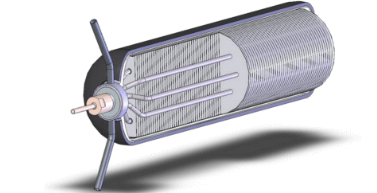
\includegraphics[width=0.4\textwidth,height=0.25\textheight,keepaspectratio]{img/disenos/notas_2007_high_density_hydrogen_storage_prototipo2.png} &
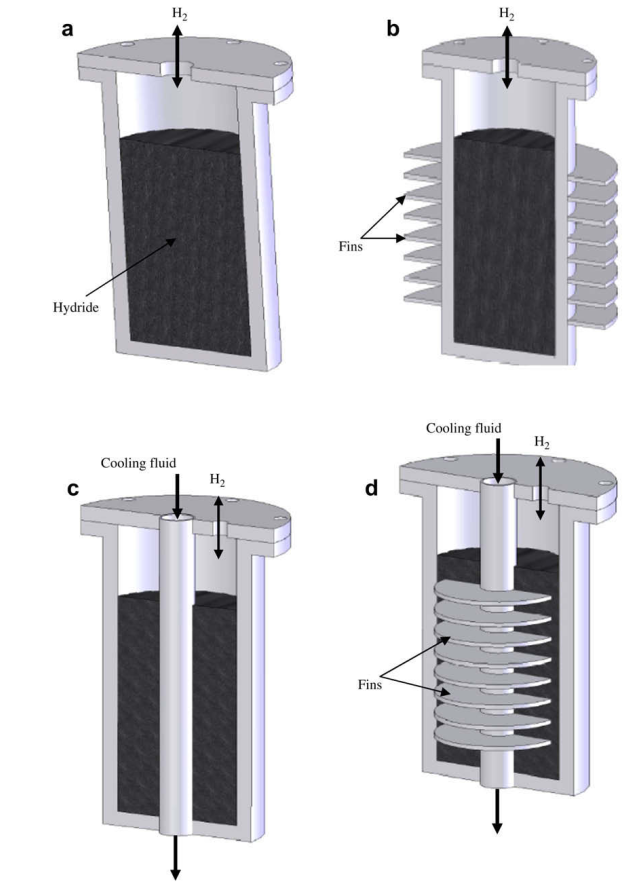
\includegraphics[width=0.4\textwidth,height=0.25\textheight,keepaspectratio]{img/disenos/notas_2008_optimization_of_hydrogen_storage_mht_Esquema_MHT_utilizados.png} \\[-0.5ex]
\small{(a) Reactor NaAlH$_4$ (2007)} & \small{(b) Configuraciones con aletas (2008)} \\[1ex]
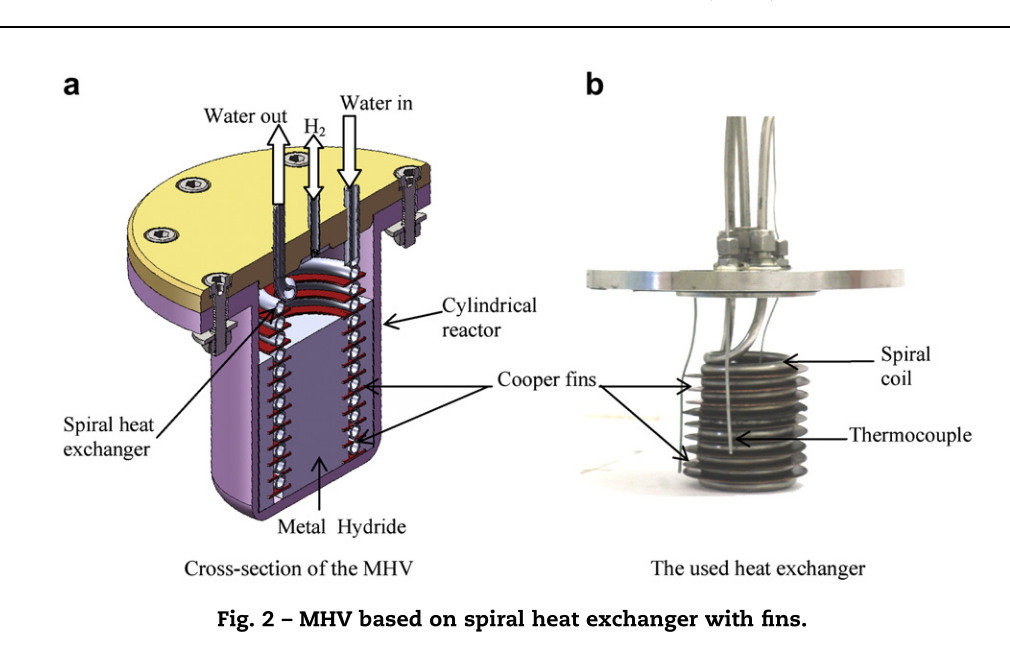
\includegraphics[width=0.4\textwidth,height=0.25\textheight,keepaspectratio]{img/disenos/notas_2010_Experimental_study_metal_hydride_vessel_based_on_finned_spiral_heat_exchanger_MHV.png} &
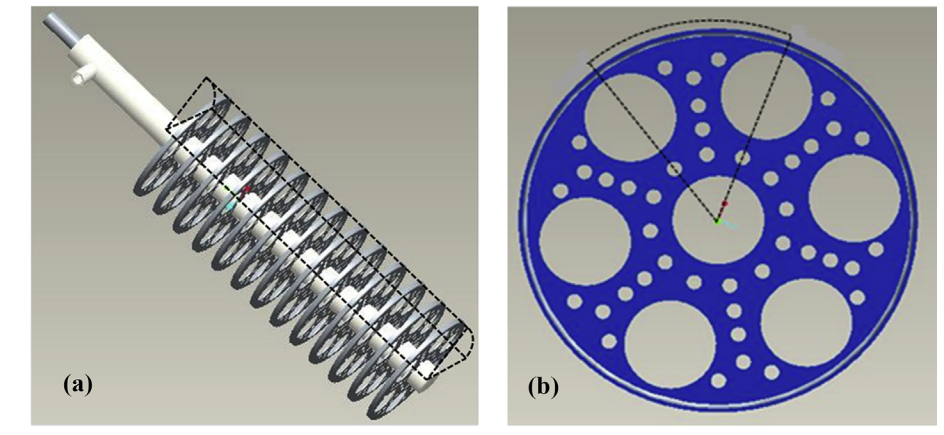
\includegraphics[width=0.4\textwidth,height=0.25\textheight,keepaspectratio]{img/disenos/notas_2015_effects_of_head_exchanger_desing_on_the_perfomace_of_solid_state_hydrogen_storage_holes.png} \\[-0.5ex]
\small{(c) Intercambiador espiral (2010)} & \small{(d) Aletas circulares (2015)} \\[1ex]
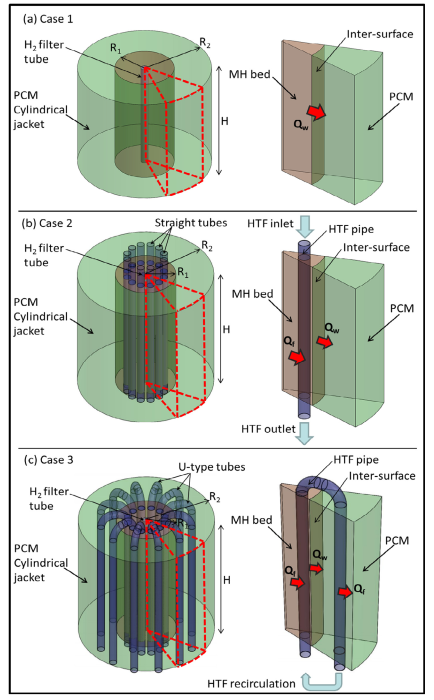
\includegraphics[width=0.4\textwidth,height=0.25\textheight,keepaspectratio]{img/disenos/notas_2017_impact_of_using_heat_transfer_fliud_pipe_tanks_geometria_var.png} &
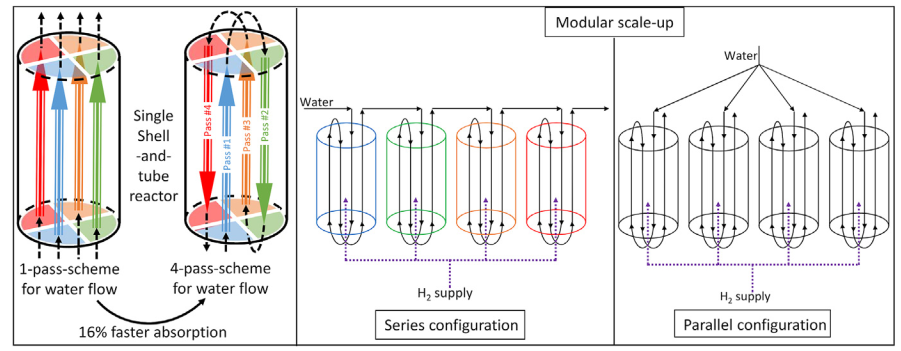
\includegraphics[width=0.4\textwidth,height=0.25\textheight,keepaspectratio]{img/disenos/notas_2023_Desing_modular_scale_up_modular.png} \\[-0.5ex]
\small{(e) Tubos HTF con PCM (2017)} & \small{(f) Diseño modular (2023)}
\end{tabular}
\caption{Comparativa de Configuraciones de Diseño de Tanques MH}\label{fig:disenos-comparativa}
\end{figure}

\clearpage

\begin{figure}[p]
\centering
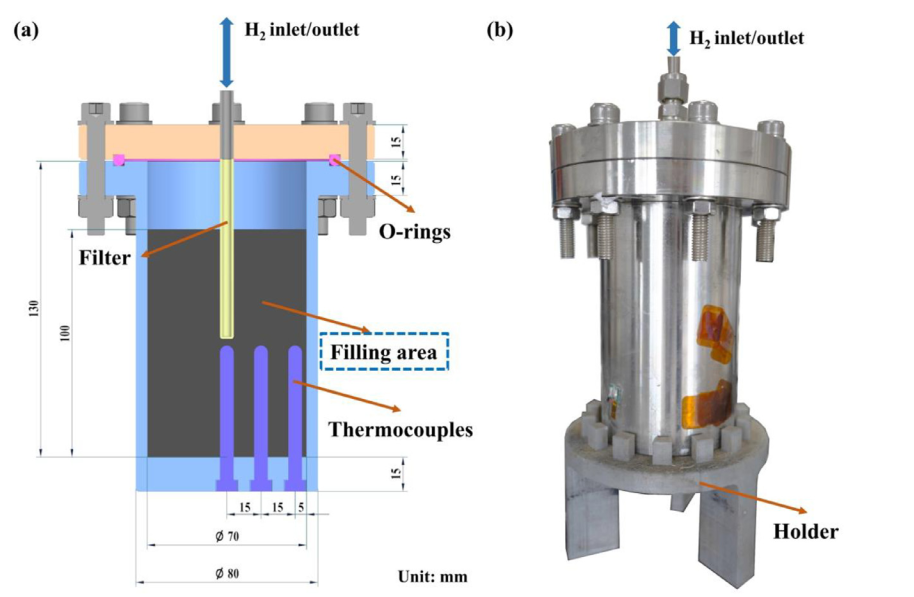
\includegraphics[width=0.75\textwidth,height=0.4\textheight,keepaspectratio]{img/disenos/notas_2024_The_relationship_between_thermal_management_tank.png}
\caption{Optimización del Diseño de Gestión Térmica (Chen et al., 2024)}\label{fig:optimizacion-termica}
\end{figure}

\FloatBarrier

\section{Justificación de la Selección de MH y Geometría}

Basándonos en el análisis comparativo de los estudios revisados y la matriz de selección, se pueden establecer las siguientes conclusiones:

\begin{enumerate}
\item \textbf{Material MH Óptimo:}
    \begin{itemize}
    \item El $\text{LaNi}_5$ demuestra ser una opción equilibrada para aplicaciones estacionarias debido a:
        \begin{itemize}
        \item Presiones y temperaturas de operación moderadas (5--15 bar, 298--350K)
        \item Buena cinética de absorción/desorción
        \item Estabilidad cíclica demostrada
        \end{itemize}
    \item Para aplicaciones de alta densidad, el $\text{NaAlH}_4$ ofrece mayor capacidad pero requiere condiciones más exigentes
    \end{itemize}

\item \textbf{Geometría Recomendada:}
    \begin{itemize}
    \item La configuración de \textbf{tubo helicoidal} emerge como la opción más eficiente para la gestión térmica
    \item Ofrece el mejor compromiso entre:
        \begin{itemize}
        \item Máxima área de transferencia de calor
        \item Distribución uniforme de temperatura
        \item Tiempo de carga/descarga reducido
        \end{itemize}
    \item La penalización en volumen de MH se compensa con la mayor eficiencia operativa
    \end{itemize}

\item \textbf{Consideraciones Adicionales:}
    \begin{itemize}
    \item La integración de PCM puede ser beneficiosa para aplicaciones que requieran recuperación de calor
    \item El uso de aletas incrementa la conductividad térmica efectiva del lecho
    \item La complejidad del diseño debe equilibrarse con la capacidad de fabricación disponible
    \end{itemize}
\end{enumerate}

\end{document}